% qec_beamer.tex
\documentclass[10pt]{beamer}
\usetheme{Madrid}
\usecolortheme{dove}
\usepackage{subcaption}
\usepackage{amsmath,amssymb,graphicx}
\usepackage{hyperref}
\usepackage{physics} % for \ket, \bra, \tr
\title[Quantum Error Correction]{Quantum Error Correction and Entanglement Purification}
\author[Tanay, Jay, Rajwardhan]{Tanay Bhat \and Jay Mehta \and Rajwardhan Toraskar}
\institute[IIT Bombay]{Department of Electrical Engineering\\Indian Institute of Technology, Bombay}
\date{\today}

\AtBeginSection[]{
  \begin{frame}
    \centering
    \Huge\insertsection
  \end{frame}
}

\begin{document}

% Title
\begin{frame}
  \titlepage
  \vfill
  \centering
\end{frame}

% Outline
\begin{frame}{Outline}
  \tableofcontents
\end{frame}

% Introduction
\section{Introduction}
\begin{frame}{Motivation}
  \begin{itemize}
    \item Quantum states are quite sensitive and prone to errors arising due to decoherence, imperfect application of gates and measurments.
    \item To combat these errors, two main strategies are employed:
      \begin{itemize}
        \item \textbf{Entanglement purification} — Use multiple noisy entangled pairs to generate a few high-fidelity pairs.
        \item \textbf{Quantum error correction (QEC)} — encode logical qubits into many physical qubits to detect and correct errors.
      \end{itemize}
    \item In this PPT, we shall analyse the 3-bit and 9-bit Shor codes for QEC and also look at the BBPSSW protocol for entanglement purification.
  \end{itemize}
\end{frame}

% Quantum errors
\section{Quantum Errors}
\begin{frame}{Types of Quantum Errors}
  Common categories:
  \begin{itemize}
    \item \textbf{Coherent errors}: Systematic over/under rotations (unitary). Generally arise due to incorrect operation of gates.
    \item \textbf{Environmental decoherence}: Coupling to the environment leads to loss of coherence.
    \item \textbf{Loss / leakage / measurement / initialization errors}.
  \end{itemize}
\end{frame}

\subsection{Coherent errors}
\begin{frame}{Coherent errors}
  Small rotation \(U = e^{i\epsilon \sigma_x}\) applied to a qubit \(N\) times:
  \[
    \ket{\psi} = \bigl(e^{i\epsilon \sigma_x}\bigr)^{\otimes N}\ket{0}
           = \cos(N\epsilon)\ket{0} + i\sin(N\epsilon)\ket{1}.
  \]
  Measurement probabilities:
  \[
    P(\ket{0})=\cos^2(N\epsilon)\approx 1-(N\epsilon)^2,\qquad 
    P(\ket{1})\approx (N\epsilon)^2.
  \]
  With QEC we can suppress such errors to higher orders ($O(\epsilon^2) \to O(\epsilon^6)$).
\end{frame}

\subsection{Decoherence}
\begin{frame}{Decoherence due to environment}
  Example: system entangles with environment \(\ket{e_0},\ket{e_1}\). The state of the environment flips if the qubit is \(\ket{1}\). Hence on application of the operation \(HIH\) to the state \(\ket{0} \ket{e_0}\), we get:

  \begin{equation*}
    \ket{\psi} = HIH \ket{0} \ket{e_0} = \frac{1}{2}(\ket{0}+\ket{1})\ket{e_0} + \frac{1}{2}(\ket{0}-\ket{1})\ket{e_1}.
  \end{equation*}

  We can then consider the density matrix of the combined system and trace out the environment to get the reduced density matrix of the system:

    \begin{equation*}
        \rho = \tr_E(\ket{\psi}\bra{\psi}) = \frac{1}{2} (
            \ket{0}\bra{0} + \ket{1}\bra{1}
        )
    \end{equation*}

    Hence the qubit is in a completely mixed state, i.e. it has decohered.
\end{frame}
\subsection{Loss, Leakage, Measurement and Initialization Errors}
\begin{frame}{Measurement Errors}
\textbf{Two Common Models:}
\begin{enumerate}
    \item \textbf{POVM Model:}
    \[
    F_0 = (1 - p_M)\ket{0}\bra{0} + p_M\ket{1}\bra{1}, \quad
    F_1 = (1 - p_M)\ket{1}\bra{1} + p_M\ket{0}\bra{0}
    \]
    Outcome probabilities:
    \[
    \text{Tr}(F_0\rho) = (1-p_M)\text{Tr}(A_0\rho) + p_M\text{Tr}(A_1\rho)
    \]
    Post-measurement state remains partially coherent:
    \[
    M_0 = \sqrt{1 - p_M}\ket{0}\bra{0} + \sqrt{p_M}\ket{1}\bra{1}
    \]

    \item \textbf{Bit-Flip Channel Model:}
    \[
    \rho' = (1 - p_M)\rho + p_M X\rho X
    \]
    Same measurement statistics, but projects directly to $\ket{0}$ or $\ket{1}$.
\end{enumerate}

\vspace{0.2cm}
\textit{For practical systems, both models are equivalent since qubits are reinitialized immediately after measurement.}
\end{frame}

%--------------------------------------------------
\begin{frame}{Qubit Loss}
\textbf{Definition:} Disappearance of the physical information carrier.  
\vspace{0.2cm}

\textbf{Model:}
\[
\rho \rightarrow \mathrm{Tr}_i(\rho)
\]
reduces the Hilbert space dimension.

\vspace{0.2cm}
\textbf{Implications:}
\begin{itemize}
    \item Standard QEC assumes all qubits are accessible.
    \item Requires \textbf{non-demolition detection} to identify loss events.
    \item Lost qubits can be replaced, improving resilience.
\end{itemize}
\end{frame}

%--------------------------------------------------
\begin{frame}{Initialization Errors}
\textbf{Two Types:}
\begin{enumerate}
    \item \textbf{Incoherent:} Imperfect statistical mixture
    \[
    \rho_i = (1 - p_I)\ket{0}\bra{0} + p_I\ket{1}\bra{1}
    \]
    \item \textbf{Coherent:} Slightly rotated pure state
    \[
    \ket{\psi_i} = \alpha\ket{0} + \beta\ket{1}, \quad |\beta|^2 \ll 1
    \]
\end{enumerate}

\vspace{0.2cm}
\textbf{Effect:} Reduces state preparation fidelity and increases measurement errors.
\end{frame}

%--------------------------------------------------
\begin{frame}{Qubit Leakage}
\textbf{Leakage:} Escape from the computational subspace $\{\ket{0}, \ket{1}\}$ into higher levels.
\[
U\ket{0} = \alpha\ket{0} + \beta\ket{1} + \gamma\ket{2}
\]

\textbf{Consequences:}
\begin{itemize}
    \item Violates two-level assumption.
    \item Causes extra decoherence if $\ket{2}$ decays quickly.
\end{itemize}

\textbf{Mitigation:}
\begin{itemize}
    \item Non-demolition verification of qubit state.
    \item Pulse refocusing to bring population back to logical subspace.
    \item Post-fabrication qubit screening.
\end{itemize}
\end{frame}

% 3-qubit code
\section{3-Qubit Bit-Flip Code}
\begin{frame}{3-Qubit Bit-Flip Code — Encoding}
  Logical codewords:
  \[
    \ket{0}_L=\ket{000},\qquad \ket{1}_L=\ket{111}.
  \]
  Encode an arbitrary qubit \(\ket{\psi}=\alpha\ket{0}+\beta\ket{1}\) as
  \[
    \ket{\psi}_L=\alpha\ket{000}+\beta\ket{111}.
  \]
 
  This code is able to correct for any single bit-flip error.
\end{frame}

\begin{frame}{Syndrome extraction \& correction}
  Use two ancillas (parity checks). Syndrome table:
  \[
    \begin{array}{c|c}
      \text{Syndrome} & \text{Correction} \\ \hline
      00 & \text{No error} \\
      01 & X_3 \\
      10 & X_2 \\
      11 & X_1
    \end{array}
  \]
  Circuit: encode with two CNOTs, measure ancillas, apply conditional \(X\).
\end{frame}

\begin{frame}{Error suppression (coherent small rotations)}
  For \(U=e^{i\epsilon \sigma_x}\) on each physical qubit:
  \[
    E = U^{\otimes 3} = c_0\,\sigma_I\sigma_I\sigma_I
      + c_1\,(\sigma_x\sigma_I\sigma_I + \dots) + c_2(\dots) + c_3\,\sigma_x\sigma_x\sigma_x,
  \]
  where
  \[
    c_0=\cos^3\epsilon,\quad c_1=i\cos^2\epsilon\sin\epsilon,\quad c_2=-\cos\epsilon\sin^2\epsilon,\quad c_3=-i\sin^3\epsilon.
  \]
  Unencoded fidelity: \(F_{\text{unencoded}}=\cos^2\epsilon\approx 1-\epsilon^2\).
  
  After post-selecting the no-error syndrome, encoded fidelity:
  \[
    F_{\text{encoded}}\approx 1-\epsilon^6.
  \]
  (Error reduced from \(O(\epsilon^2)\) to \(O(\epsilon^6)\).)
\end{frame}

% Shor code
\section{9-Qubit Shor Code}
\begin{frame}{Shor 9-Qubit Code — Logical states}
  Combine phase-flip and bit-flip repetition codes.
  \[
    \ket{0}_L = \frac{1}{2\sqrt{2}} ( \ket{000}+\ket{111} )^{\otimes 3},\quad
    \ket{1}_L = \frac{1}{2\sqrt{2}} ( \ket{000}-\ket{111} )^{\otimes 3}.
  \]
  Each block of 3 corrects an \(X\) error; inter-block checks correct \(Z\) errors.
\end{frame}

\begin{frame}{How it protects against arbitrary single-qubit errors}
  An arbitrary single-qubit error can be expanded in Pauli basis.
  The combined bit-flip and phase-flip checks detect and correct single-qubit \(X\), \(Z\) (and hence \(Y\)) errors.
  Coherent rotation generalization:
  \[
    E=\bigotimes_{i=1}^{9}(\cos\epsilon\,\sigma_I + i\sin\epsilon\,\sigma_x),
  \]
  followed by appropriate syndrome circuits increases logical fidelity compared to unencoded qubit.
\end{frame}

% Purification
\section{Entanglement Purification (BBPSSW)}
\begin{frame}{Communication over a noisy channel}
  One way to transmit quantum information is to share entangled pairs (e.g. Bell pairs) between sender and receiver and use teleportation. However, teleportation involves sharing a maximally entangled pair, which is hard to achieve over a noisy channel. Entanglement purification protocols use multiple noisy pairs to generate fewer high-fidelity pairs.
\end{frame}

\begin{frame}{Werner states and depolarization}
  Any two-qubit state can be depolarized to a Werner form without changing fidelity with \(\ket{\phi_{00}}\):
  \[
    \rho_W(x)= x\ket{\phi_{00}}\bra{\phi_{00}} + \frac{1-x}{4} I_4.
  \]
  Fidelity relative to \(\ket{\phi_{00}}\): \(F=\bra{\phi_{00}}\rho_W\ket{\phi_{00}}=\frac{3x+1}{4}.\)
\end{frame}

\begin{frame}{BBPSSW protocol (recurrence)}
  Starting with pairs of fidelity \(F>1/2\):
  \begin{enumerate}
    \item Depolarize to Werner form \(\rho_W(F)\).
    \item Take two copies; apply bilateral CNOT (A1→A2 and B1→B2).
    \item Measure target qubits (A2,B2) in \(Z\)- and \(X\)-bases; keep control pair if measurement results match.
  \end{enumerate}
\end{frame}

\begin{frame}{Fidelity update and success probability}
  After one successful purification step the surviving pair (still Werner) has fidelity
  \[
    F'=\frac{F^2 + \left(\tfrac{1-F}{3}\right)^2}{F^2 + 2F\big(\tfrac{1-F}{3}\big) + 5\big(\tfrac{1-F}{3}\big)^2},
  \]
  and the success probability is
  \[
    p_{\text{succ}} = F^2 + 2F\Big(\frac{1-F}{3}\Big) + 5\Big(\frac{1-F}{3}\Big)^2.
  \]
  Iterating increases fidelity but reduces yield (consume 2 pairs to keep 1).
\end{frame}

% Implementation
\section{Implementation \& Results}
\begin{frame}{Qiskit simulations}
  \begin{itemize}
    \item 3-qubit bit-flip and phase-error simulations: encoding, injecting error, syndrome extraction, correction, decode. Observed fidelity improvement consistent with theory (e.g. \(1-\epsilon^2 \to 1-\epsilon^6\)).
    \item 9-qubit Shor code simulation: injected single \(Z\) error, used 6 ancillas for syndrome extraction; decoded and observed restored logical state.
  \end{itemize}
  Code repository (included in report): \\
  \small \url{https://github.com/jaymehta132/QuantumErrorCorrection-EE7001}
\end{frame}

% \begin{frame}{Example figures (placeholders)}
  
% \end{frame}


%------------------------------------------------
% \begin{frame}{Overview}
% \begin{itemize}
%     \item Simulations implemented using \textbf{Qiskit}.
%     \item Demonstrated:
%     \begin{enumerate}
%         \item 3-bit bit-flip code (X error correction)
%         \item 3-bit phase error correction
%         \item 9-bit Shor code (Z error correction)
%     \end{enumerate}
%     \item All circuits and results available in the GitHub repository:
%     \begin{itemize}
%         \item \url{https://github.com/jaymehta132/QuantumErrorCorrection-EE7001}
%     \end{itemize}
%     \item Objective: Validate QEC protocols and verify theoretical fidelity improvements.
% \end{itemize}
% \end{frame}

%------------------------------------------------
\subsection{3-Bit Code for Bit-Flip Error}
\begin{frame}{3-Bit Code for Bit-Flip (X) Error}
\textbf{Process:}
\begin{enumerate}
    \item Encode logical qubit using Hadamard + 2 CNOTs.
    \item Inject bit-flip error (X gate) on one qubit.
    \item Detect error using 2 ancilla qubits and 4 CNOTs.
    \item Apply conditional correction based on syndrome.
    \item Decode and measure final qubit.
\end{enumerate}

\vspace{0.3cm}
\textbf{Result:} Measured state “001” with probability 1 — successful correction.

\begin{figure}
  
  \centering
  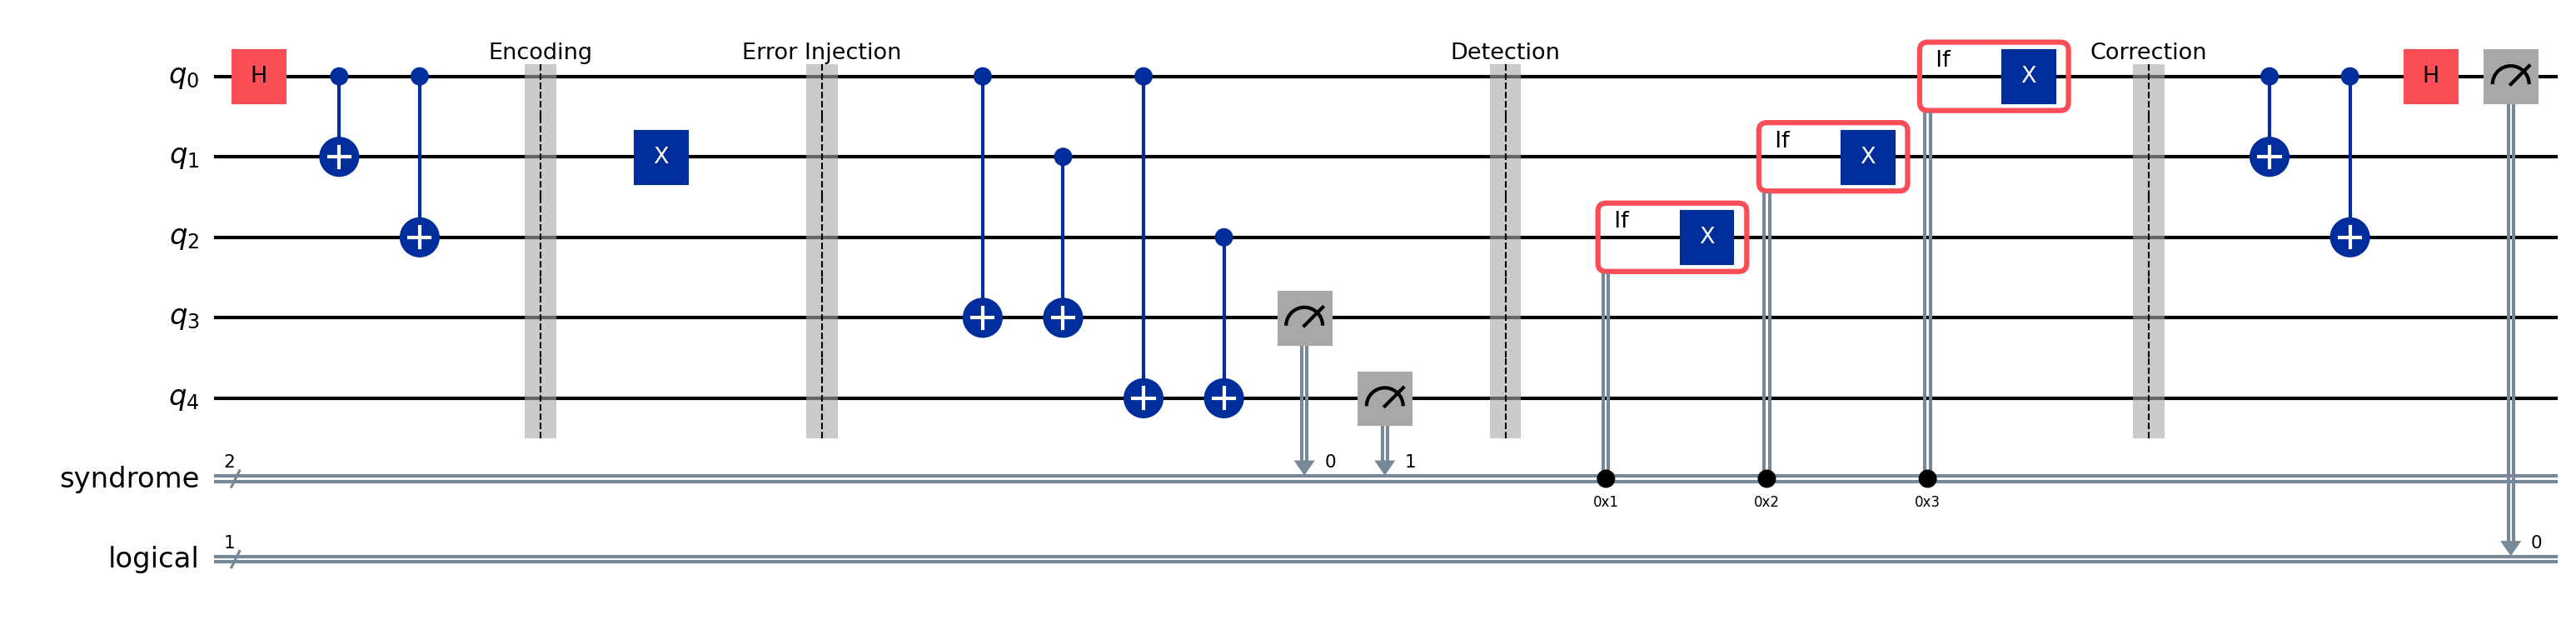
\includegraphics[width=0.7\textwidth]{../../Codes/results/3bitCode/3bitCodeCircuit.png} \\[4pt]
  \caption{3-bit Code Circuit for X Error}
\end{figure}
\end{frame}

%------------------------------------------------
\begin{frame}{3-Bit Code: X Error Results}
\begin{itemize}
    \item Histogram confirms complete recovery of logical qubit.
    \item Fidelity maintained post-correction.
    \item Demonstrates robustness of simple repetition code for single X-error.
\end{itemize}

\vspace{0.3cm}
\begin{figure}
    \centering
    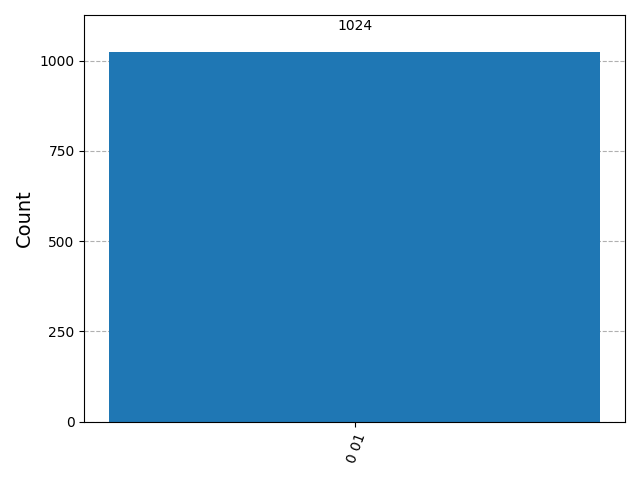
\includegraphics[width=0.55\textwidth]{../../Codes/results/3bitCode/3bitCodeHistogram.png}
    \caption{3-bit Code Results for X Error}
    \label{fig:3bitCodeHistogram}
\end{figure}
% \centering
% 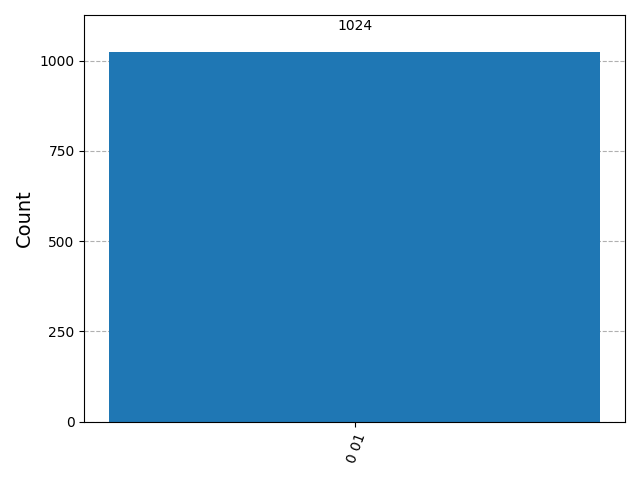
\includegraphics[width=0.55\textwidth]{../../Codes/results/3bitCode/3bitCodeHistogram.png} \\[4pt]
% {\scriptsize Fig. 2: 3-bit Code Results for X Error}
\end{frame}

%------------------------------------------------
\subsection{3-Bit Code for Phase Error}
\begin{frame}{3-Bit Code for Phase Error}
\textbf{Goal:} Verify suppression of coherent rotation errors $U = e^{i\epsilon \sigma_x}$.

\textbf{Procedure:}
\begin{itemize}
    \item Encode qubit via CNOTs.
    \item Apply small X-rotation ($\epsilon$) to all three data qubits.
    \item Measure syndrome using two ancillas.
    \item Decode and compute fidelity.
\end{itemize}

\textbf{Observation:}
\[
F_{\text{unencoded}} = 1 - \epsilon^2 \quad \text{vs.} \quad F_{\text{encoded}} = 1 - \epsilon^6
\]

\begin{figure}[h!]
    \centering

    \begin{subfigure}[b]{0.3\columnwidth}
        \centering
        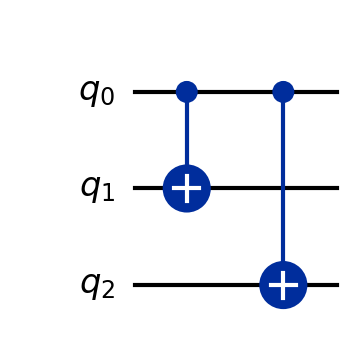
\includegraphics[width=0.75\textwidth]{../../Codes/results/3bitPhaseEC/EncodingCircuit.png}
        \caption{Encoding Circuit}
        \label{fig:3bitPhaseECCircuit}
    \end{subfigure}
    \hfill
    \begin{subfigure}[b]{0.3\columnwidth}
        \centering
        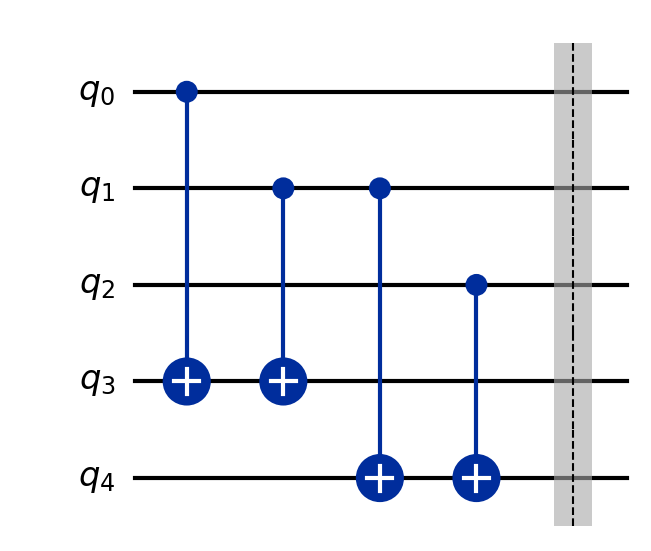
\includegraphics[width=0.75\textwidth]{../../Codes/results/3bitPhaseEC/SyndromeMeasurementCircuit.png}
        \caption{Syndrome Measurement Circuit}
        \label{fig:3bitPhaseDecodingCircuit}
    \end{subfigure}
    \hfill
    \begin{subfigure}[b]{0.3\columnwidth}
        \centering
        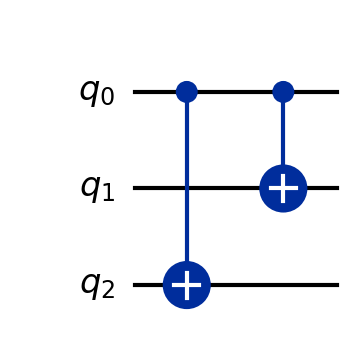
\includegraphics[width=0.75\textwidth]{../../Codes/results/3bitPhaseEC/DecodingCircuit.png}
        \caption{Decoding Circuit}
        \label{fig:3bitPhaseAncillaCircuit}
    \end{subfigure}

    \caption{3-bit Code Circuits for Phase error}
    \label{fig:three_images}
\end{figure}
\end{frame}

%------------------------------------------------
\subsection{9-Bit Shor Code for Z Error}
\begin{frame}{9-Bit Shor Code for Z Error}
\textbf{Overview:}
\begin{itemize}
    \item Protects logical qubit against arbitrary single-qubit errors.
    \item Encodes $|+\rangle$ using layered 3x3 block structure:
    \begin{itemize}
        \item Inner: Bit-flip code
        \item Outer: Phase-flip code
    \end{itemize}
    \item Inject phase-flip (Z) error on one qubit.
    \item Use 6 ancillas for syndrome extraction.
\end{itemize}

\begin{figure}[h!]
\centering
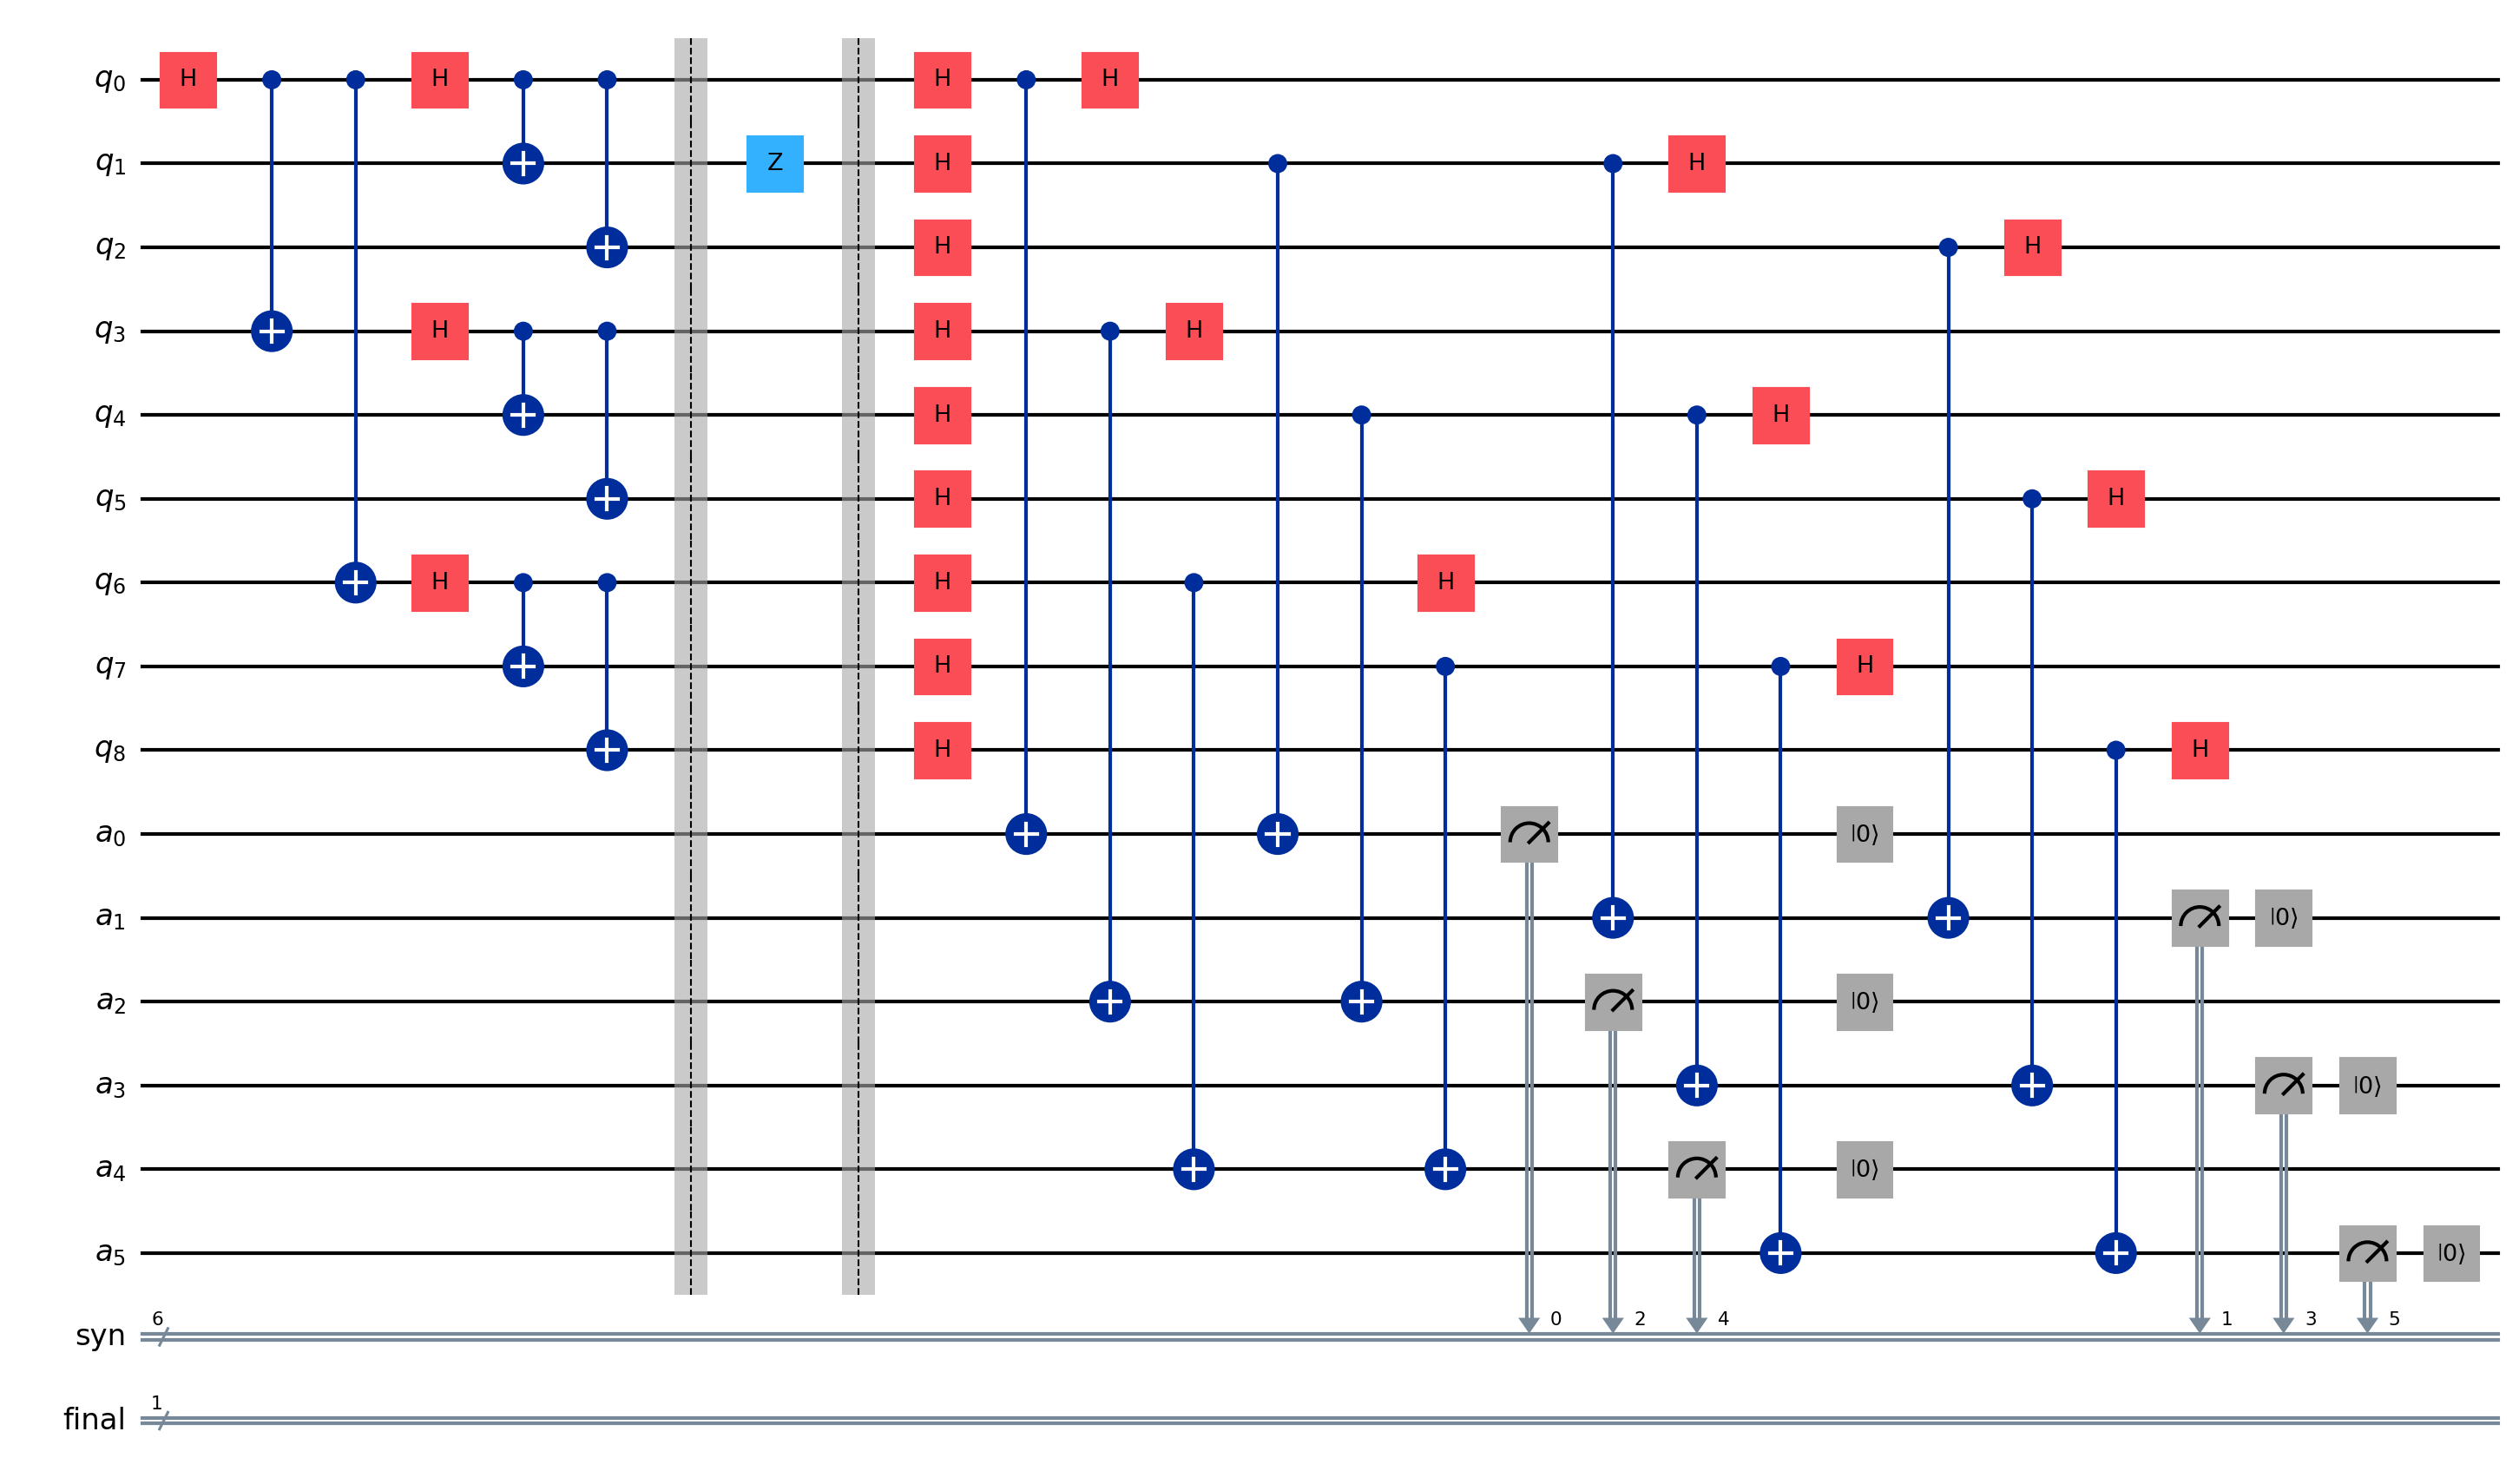
\includegraphics[width=0.55\textwidth]{../../Codes/results/9bitCode/SyndromeMeasurementCircuit.png} \\[4pt]
\caption{9-bit Shor Code — Syndrome Measurement}
\end{figure}
\end{frame}

%------------------------------------------------
\begin{frame}{9-Bit Shor Code Results}
\begin{itemize}
    \item Syndrome bits identify error location.
    \item Corrective Z operation restores logical state.
    \item Decoded qubit measured in X-basis gives deterministic “0”.
\end{itemize}

\vspace{0.2cm}
\textbf{Result:} Successful recovery of logical qubit — validates Shor code's ability to correct any single-qubit error.

\begin{figure}[h!]
  
  \centering
  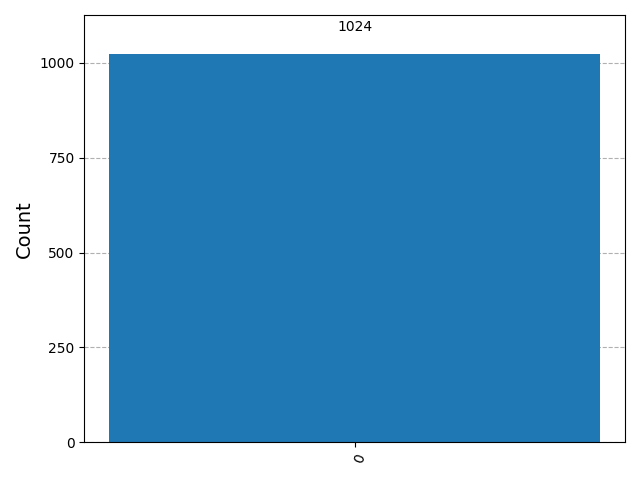
\includegraphics[width=0.5\textwidth]{../../Codes/results/9bitCode/FinalHistogram.png} \\[4pt]
  \caption{9-bit Code Results for Z Error}
\end{figure}
\end{frame}

%------------------------------------------------
\begin{frame}{Summary of Simulations}
\begin{itemize}
    \item \textbf{3-bit Code (X error):} Corrects single bit-flip errors with fidelity $\approx 1$.
    \item \textbf{3-bit Code (Phase error):} Reduces error probability from $O(\epsilon^2)$ to $O(\epsilon^6)$.
    \item \textbf{9-bit Shor Code:} Corrects arbitrary single-qubit errors using nested redundancy.
\end{itemize}

\vspace{0.3cm}
\textbf{Takeaway:}
\begin{itemize}
    \item Qiskit simulations validate theoretical predictions.
    \item Demonstrate the feasibility of small-scale QEC on near-term quantum hardware.
\end{itemize}
\end{frame}


% Conclusion
\section{Conclusion}
\begin{frame}{Conclusions \& Outlook}
  \begin{itemize}
    \item QEC and entanglement purification are foundational for fault-tolerant quantum computing and long-distance quantum communication.
    \item Simple codes (3- and 9-qubit) illustrate suppression of coherent errors and correction of arbitrary single-qubit errors.
    \item Real devices: gate errors, measurement noise, and leakage limit achievable fidelities; fault-tolerance requires concatenation or more advanced topological/subsystem codes and careful experimental engineering.
  \end{itemize}
\end{frame}

% References
\begin{frame}[allowframebreaks]{References}
  \begin{thebibliography}{9}
    \bibitem{devitt2013}
      S. J. Devitt, W. J. Munro, K. Nemoto, ``Quantum error correction for beginners,'' Reports on Progress in Physics, 2013.
    \bibitem{dur2007}
      W. D\"ur and H.-J. Briegel, ``Entanglement purification and quantum error correction,'' Reports on Progress in Physics, 2007.
    % \bibitem{report}
    %   Project report (uploaded): ``Quantum Error Correction (EE7001)'' by Tanay Bhat et al. :contentReference[oaicite:2]{index=2}
  \end{thebibliography}
\end{frame}

\end{document}
